\section{Finding Multiple Objects}

\todo[inline, color=red!50]{Add topic: Viola Jones (face detection)}

The core problem is efficiently scanning many positions for possible faces. Potential approaches include:
\begin{itemize}
	\item {\color{DodgerBlue4} Features}
	\item {\color{DodgerBlue4} Classifier}
	\item {\color{DodgerBlue4} Sliding Window}
	\item {\color{Firebrick1} Haar Features}
	\item {\color{Firebrick1} Boosting}
	\item {\color{Firebrick1} Cascaded Classifiers}
\end{itemize}

\subsection{Boosting}
Given input training data with weights, at each step $t \in 1..T$, train a weak classifier.
Let it classify the training data and increase the weight on incorrectly classified samples.
The final strong classifier $F(x)$ is a weighted, linear combination of the weak classifiers.
\[
F(x) = \alpha_1 f_1(x) + \alpha_2 f_2(x) + \alpha_2 f_2(x) + \dots
\]
The weak classifier $h_j (\theta)$ is defined with features $f$, threshold $\theta$, and parity $p_j$:
\[
h_j (\theta) = \begin{cases}
1 & p_j f_j < p_j \theta_j \\
0 & \text{otherwise}
\end{cases}
\]

\subsection{Haar Features}
To avoid computationally intensive filter responses, Haar features use simple filters with $-1$ or $1$ in masks.
Features are calculated on sliding sub-windows (e.g., $24\times24$ pixels) using integral images for fast computation.
The humongous size of features can be evaluated efficiently using integral images.

\begin{figure}[h]
	\centering
	\begin{subfigure}[t]{0.45\linewidth}
		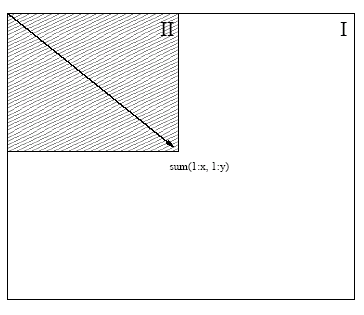
\includegraphics[width=\linewidth]{img/integral_image}
		\caption{Integral Image Visualization}
		\label{fig:integralimage}
	\end{subfigure}
	\begin{subfigure}[t]{0.45\linewidth}
	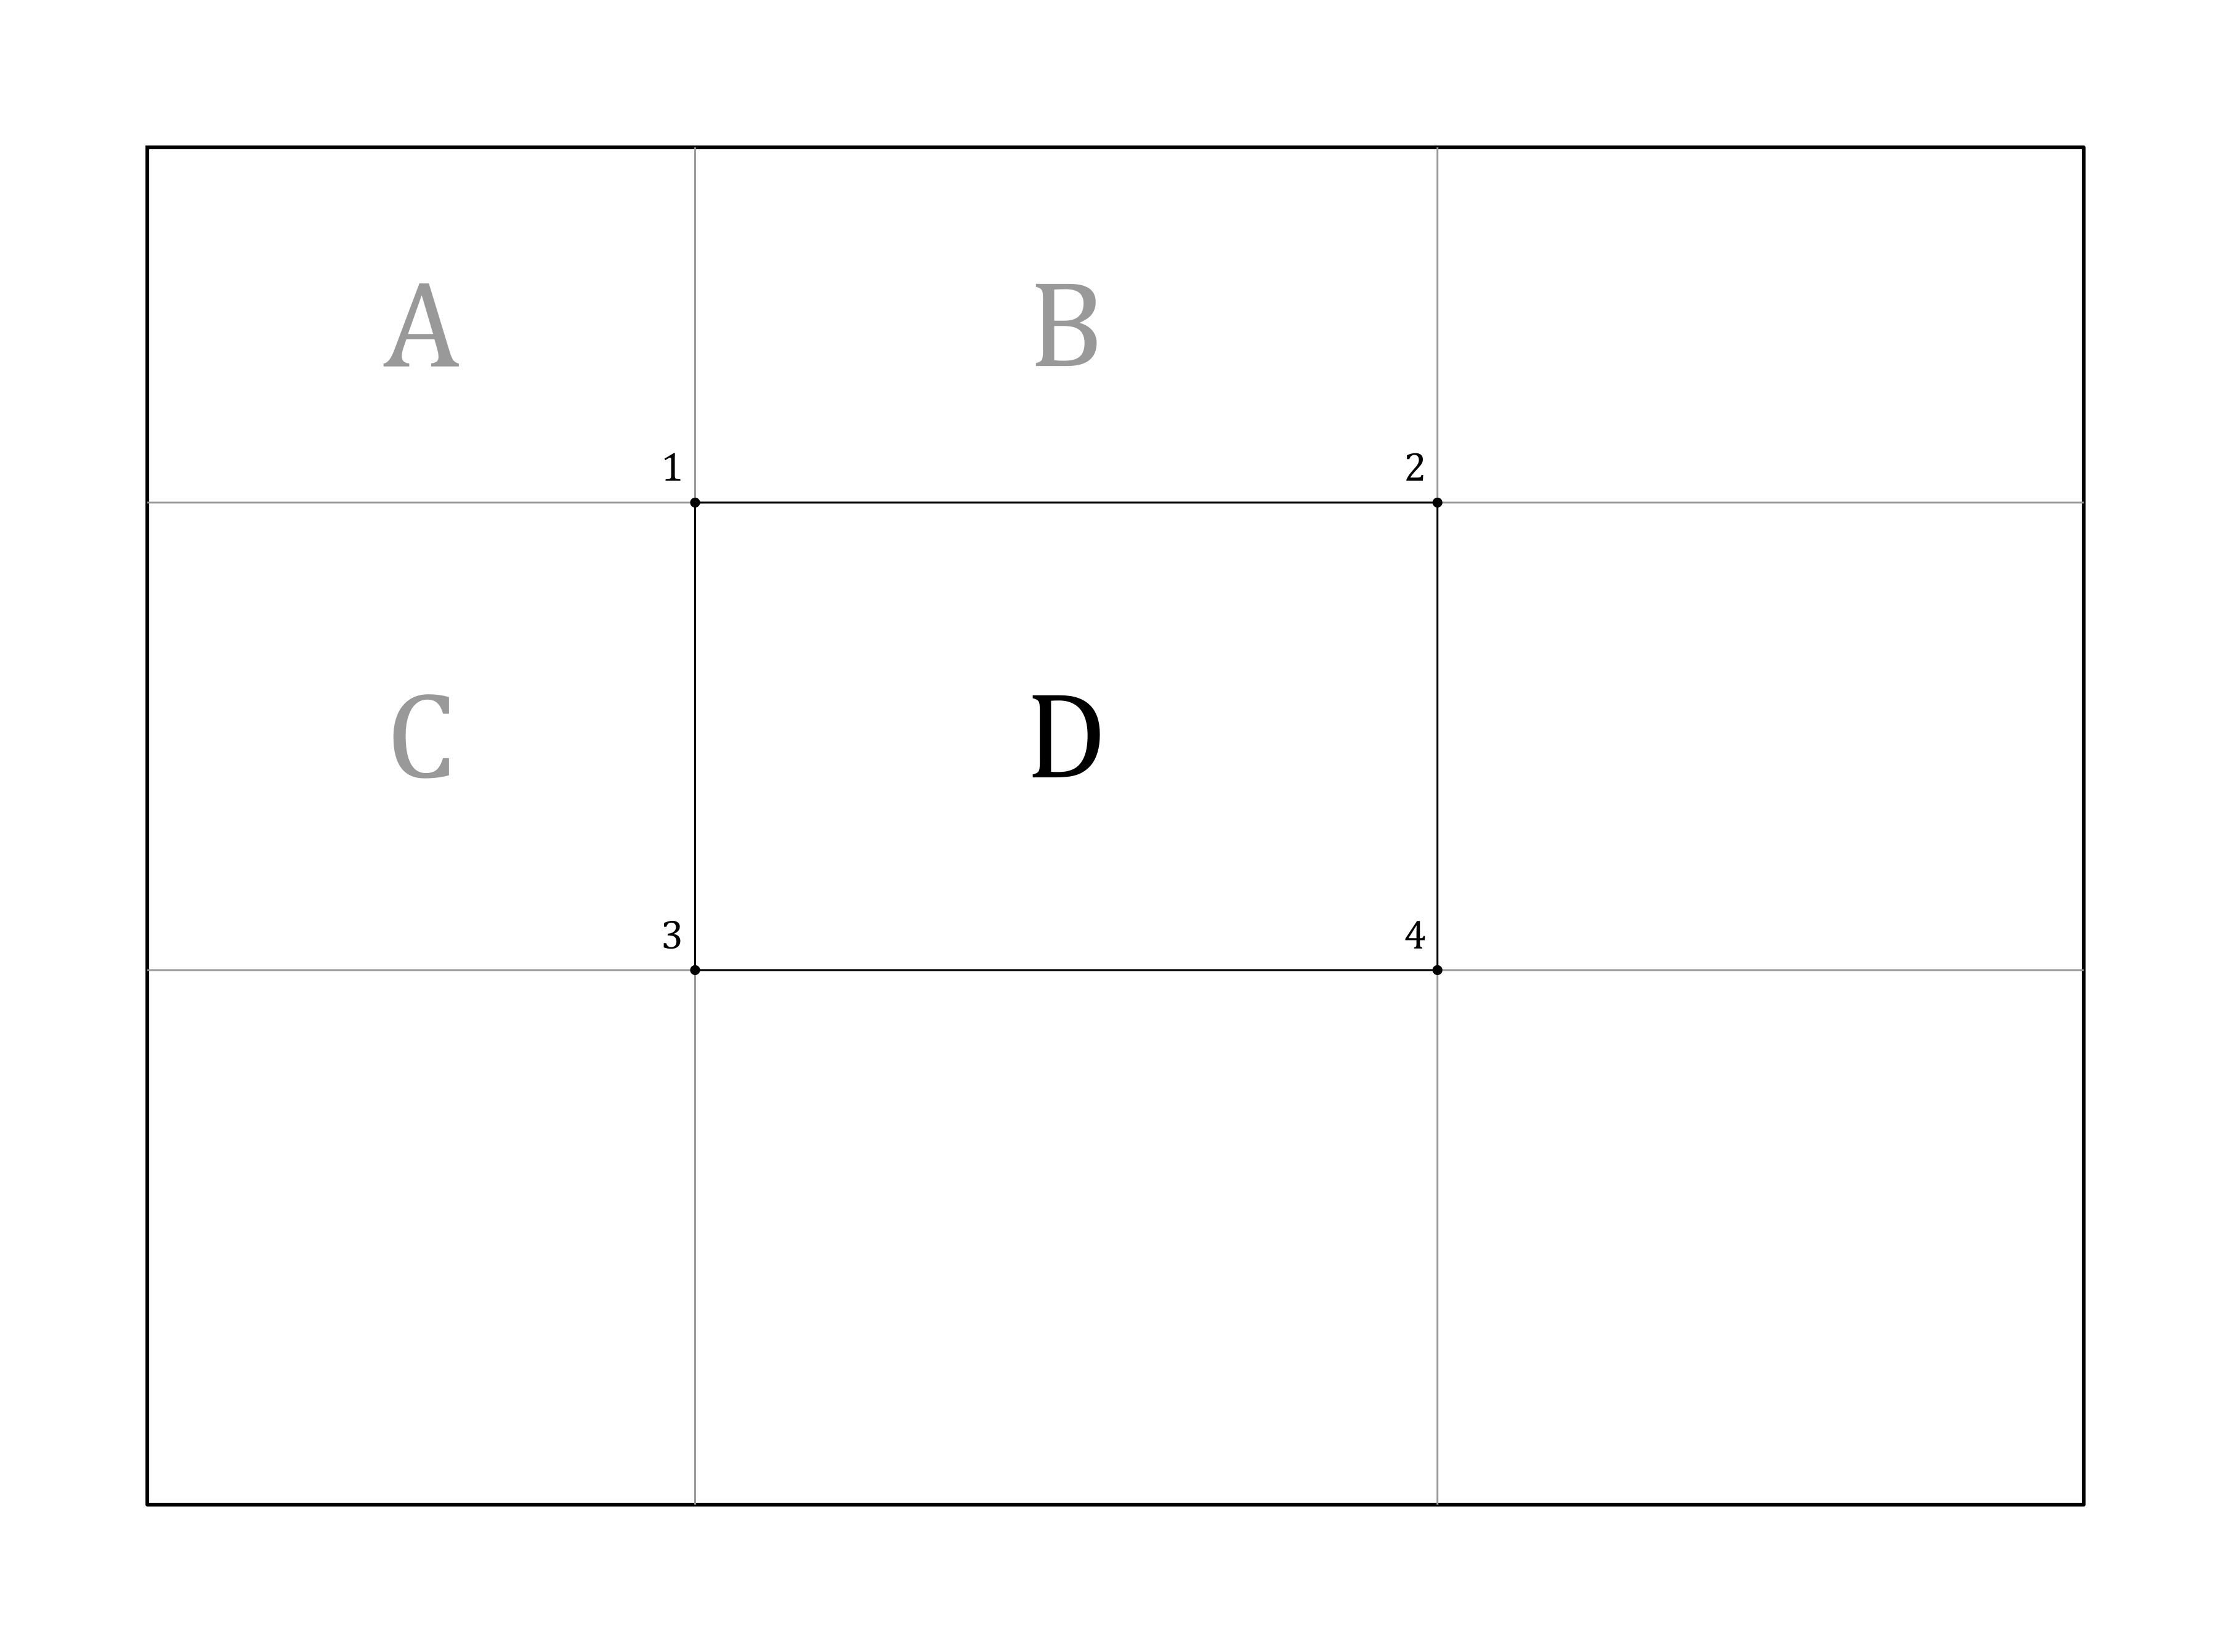
\includegraphics[width=\linewidth]{img/integral_image_haar}
	\caption{Calculating Haar Features with Integral Image}
	\label{fig:integralimagehaar}
	\end{subfigure}
\end{figure}

\subsection{Face Detection}
The challenge is evaluating thousands of possible position or scale combinations efficiently, with true faces being rare.
A classifier with a high \emph{true} positive rate (85\%-95\%) and a low \emph{false} positive rate ($10^{-5}-10^{-6}$) is used in a cascade.
False results are rejected early in the processing.

\begin{figure}[h]
	\centering
	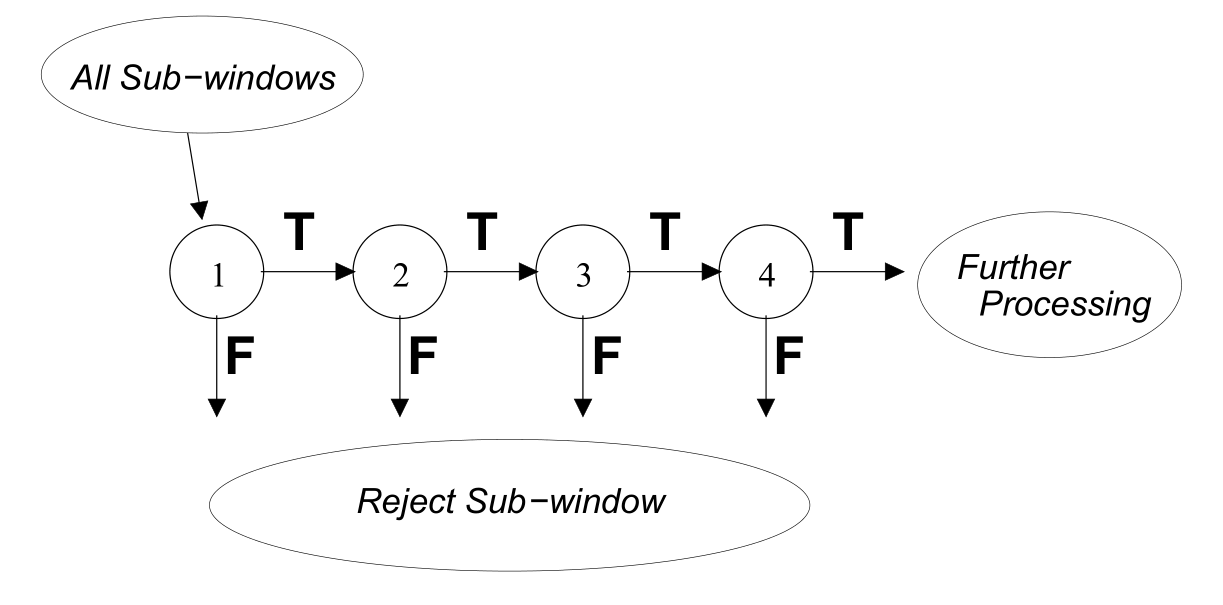
\includegraphics[width=0.6\linewidth]{img/cascade_classifier_approach}
	\caption{Cascade Classifier Approach}
\end{figure}

\subsection{HOG for Human Detection}
Detection pipeline:
\begin{itemize}
	\item Calculate HOG Descriptors
	\item Collect HOGs in Detection Window
	\item Use Linear SVM for Person or Non-Person Classification
\end{itemize}

\begin{figure}[h]
	\centering
	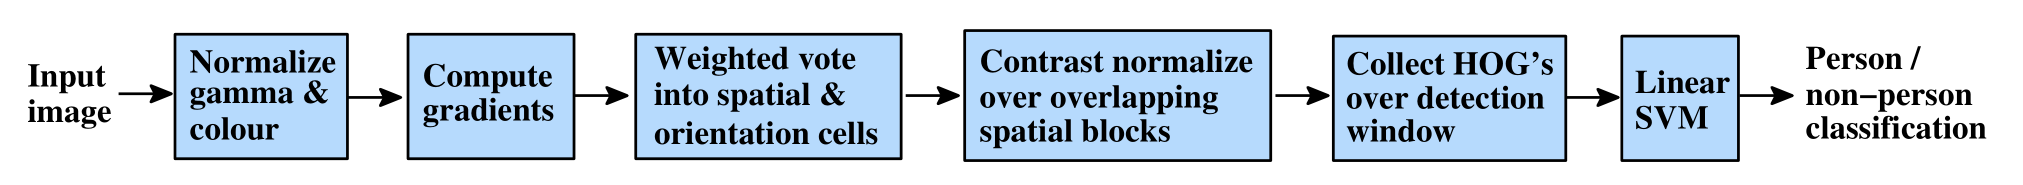
\includegraphics[width=0.8\linewidth]{img/hog_human_detection}
	\caption{HOG for Human Detection}
\end{figure}

\subsection{OverFeat}
Combining Classification, Localization, and Detection involves:
\begin{itemize}
	\item Classification
	\begin{itemize}
		\item CNN
		\item Sliding Windows applied at every possible pixel and at multiple scales
		\item Subsampling factor of 12
	\end{itemize}
	\item Localisation
	\begin{itemize}
		\item Generate Bounding Box Prediction as a Regression Problem
		\item Uses the first five layers in the CNN
	\end{itemize}
	\item Detection
	\begin{itemize}
		\item Combine Classification and Localisation
		\item Merge and accumulate bounding boxes
	\end{itemize}
\end{itemize}

\begin{figure}[h]
	\centering
	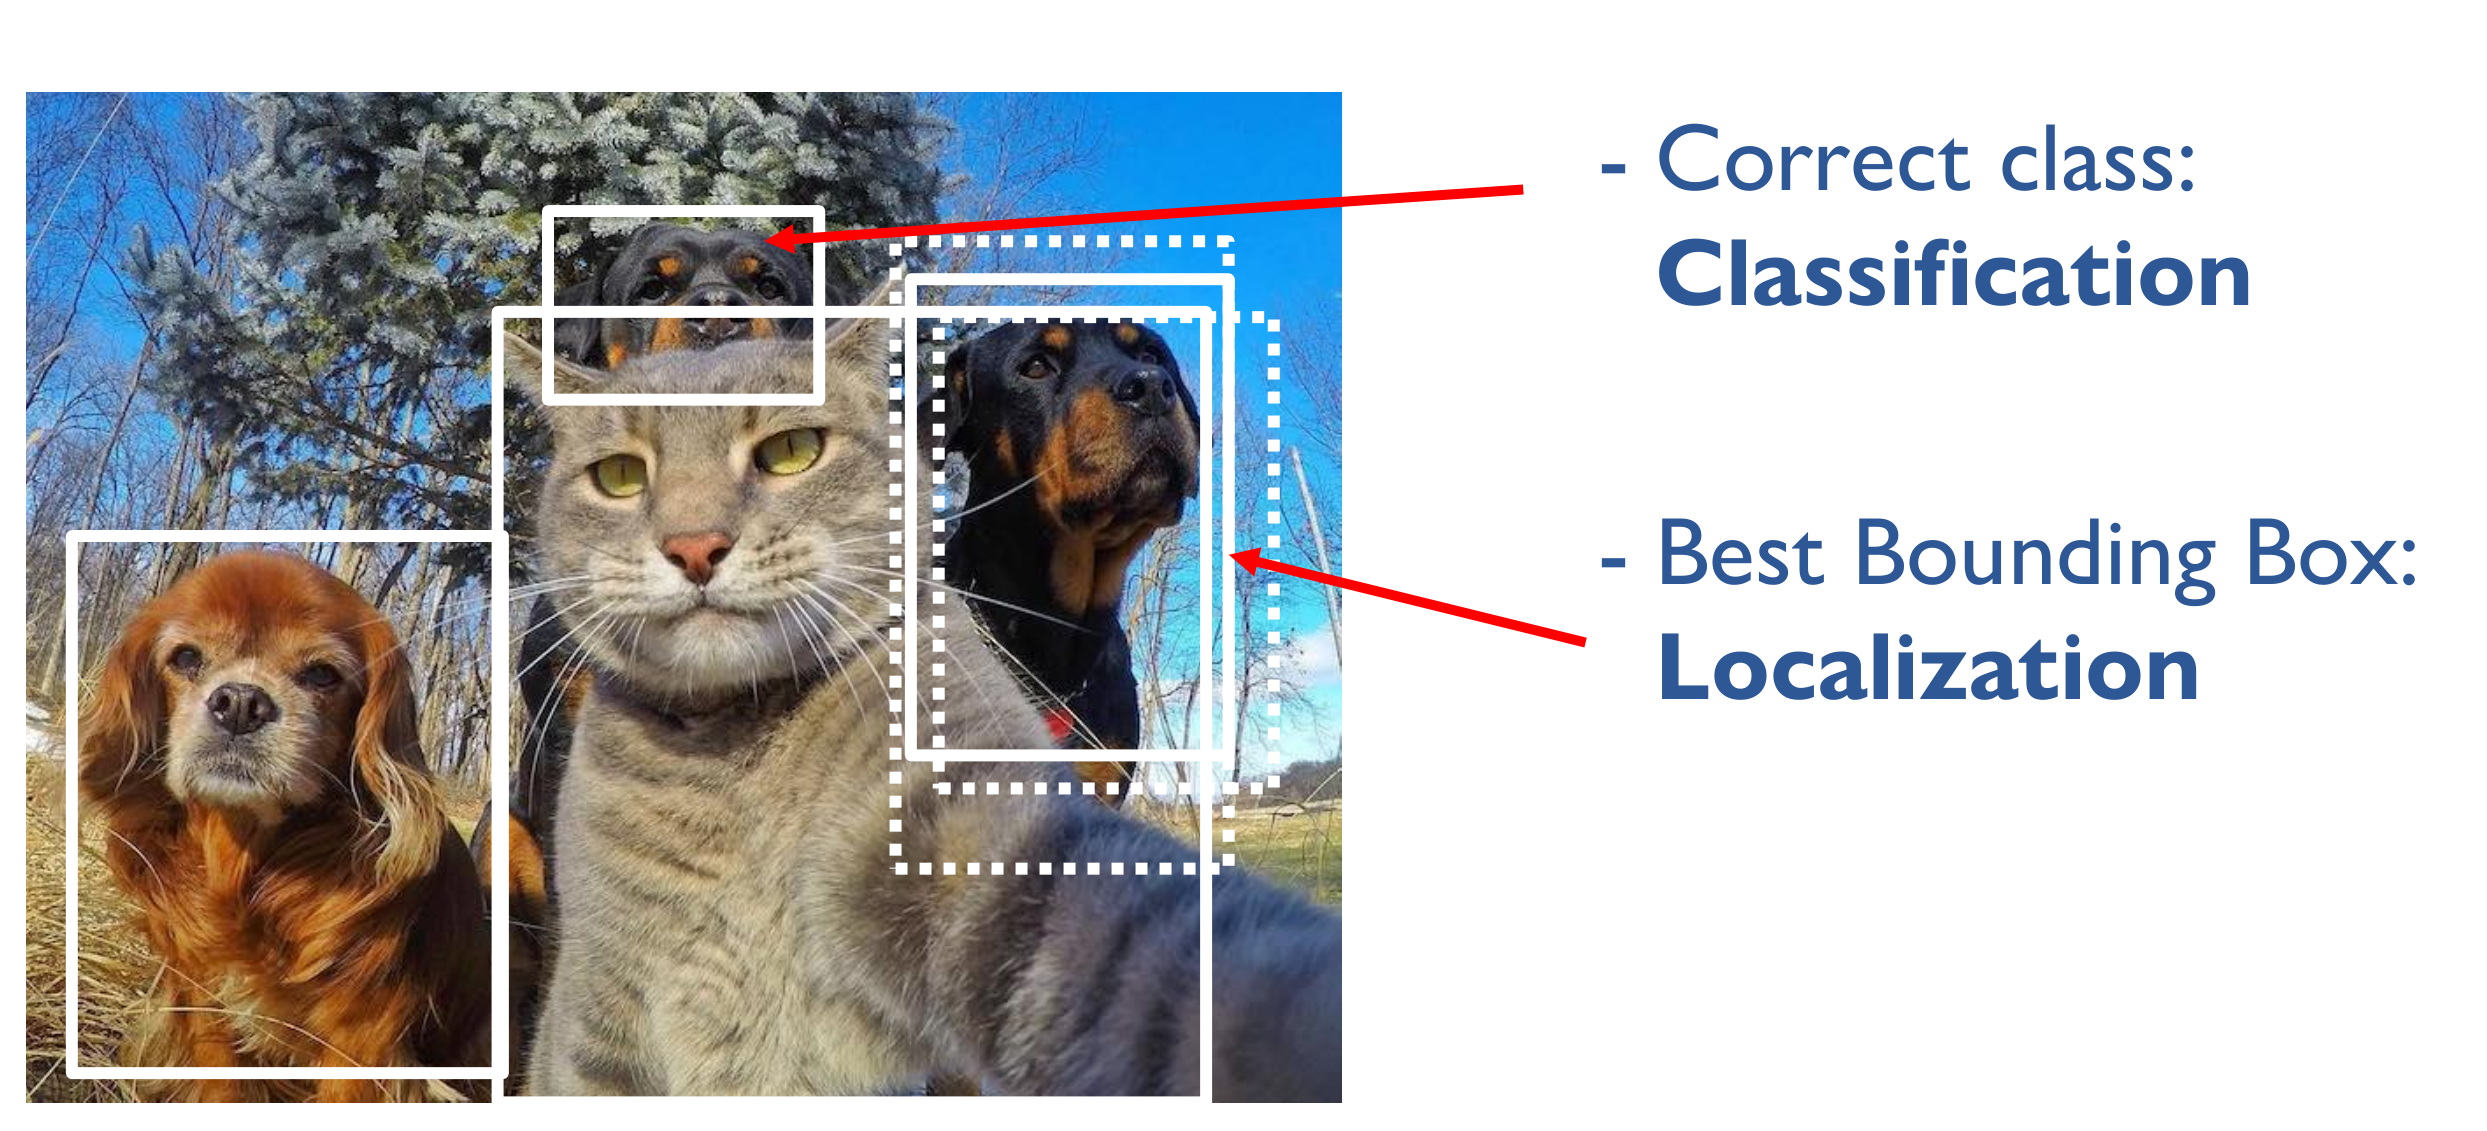
\includegraphics[width=0.7\linewidth]{img/classification_localisation}
	\caption{Classification and Localisation Visualization}
	\label{fig:classificationlocalisation}
\end{figure}

Sliding windows have the drawback of a huge number of different positions and sizes that need evaluation.
A better idea is to find image regions likely to contain an object, called region proposals.

\subsection{R-CNN}
Extract region proposals, compute CNN features, and classify regions using SVM.

\begin{figure}[h]
	\centering
	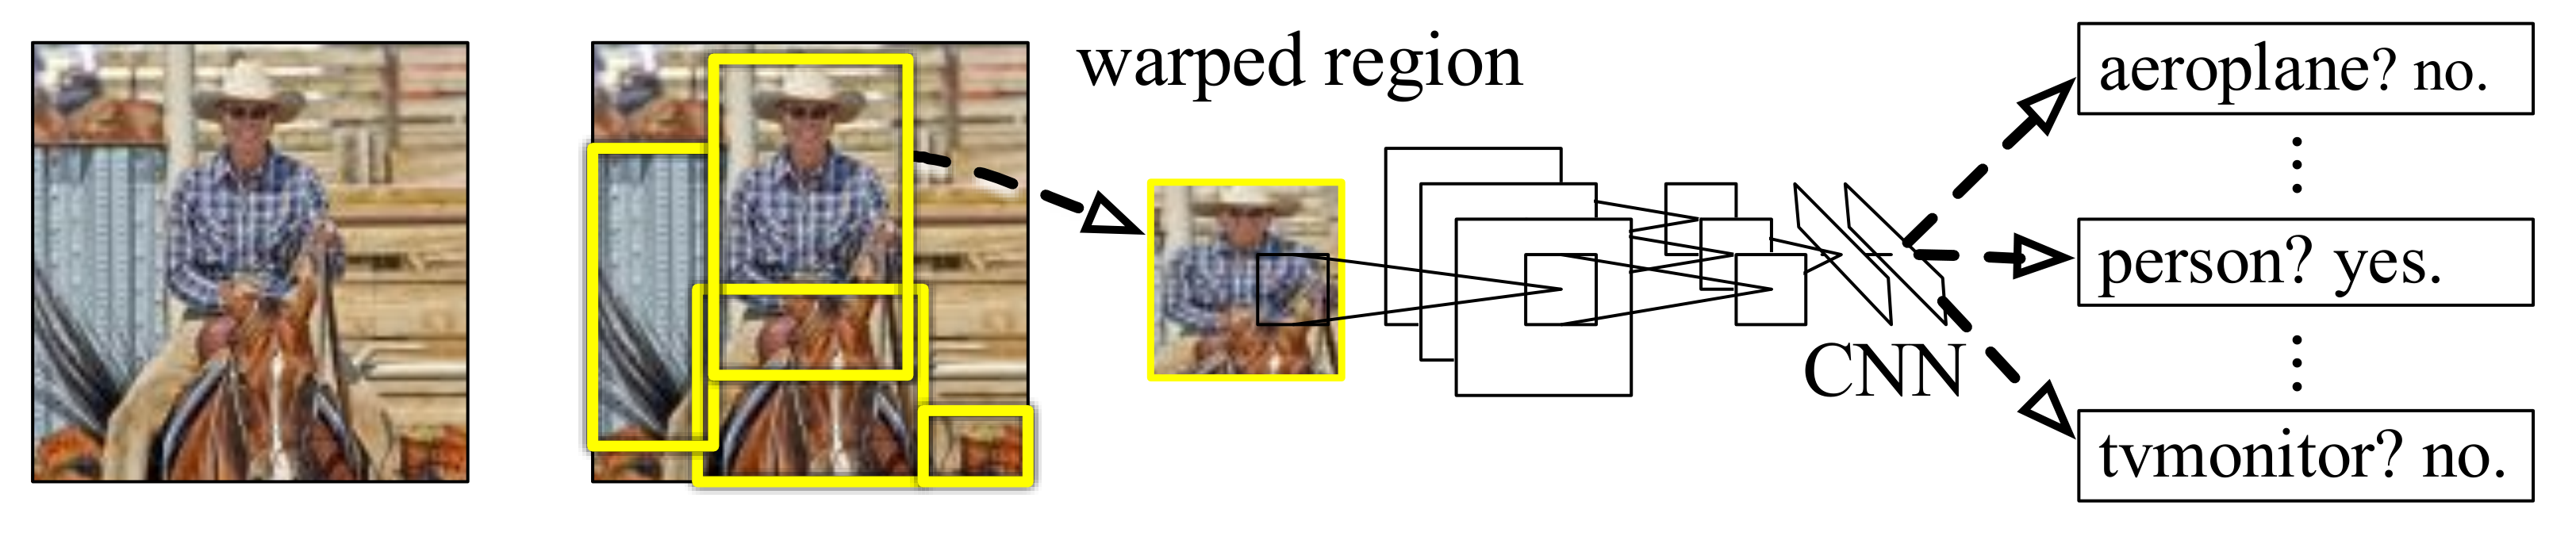
\includegraphics[width=0.7\linewidth]{img/r-cnn}
\end{figure}

\begin{figure}[h]
	\centering
	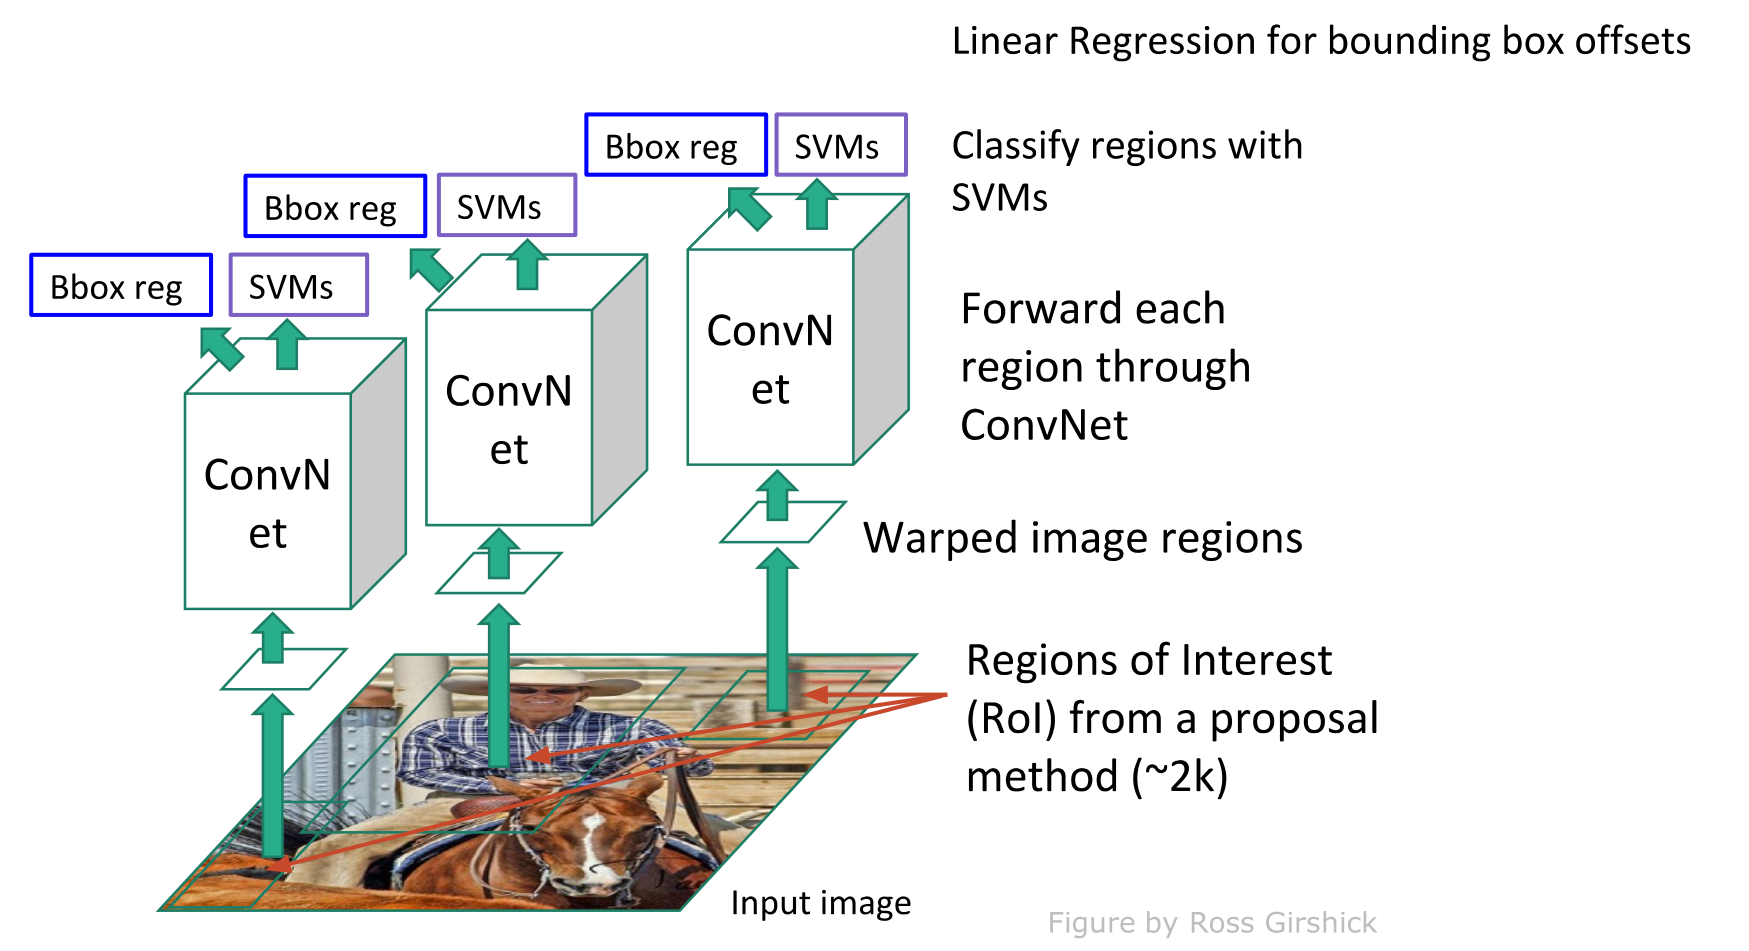
\includegraphics[width=0.7\linewidth]{img/r-cnn_structure}
	\caption{R-CNN Structure}
\end{figure}

\subsubsection{Feature Extraction}
\begin{itemize}
	\item Proposal regions are warped to $227\times 227$ pixel images
	\item 4096 Features from $227\times 227$ RGB Image using five Convolutional and two fully connected layers from AlexNet Architecture
	\item Supervised pre-training on the ILSVRC2012 classification data set
	\item Domain-specific fine-tuning continues training on warped region proposals
\end{itemize}

\subsubsection{Classifier}
Use one linear SVM per class, considering regions with overlap of 30\% as a positive example. Treat bounding box position as a regression problem.

\subsubsection{FAST R-CNN}
Replace SVM of R-CNN with a fully connected neural network for classification of objects and refined bounding boxes.

\begin{figure}[h]
	\centering
	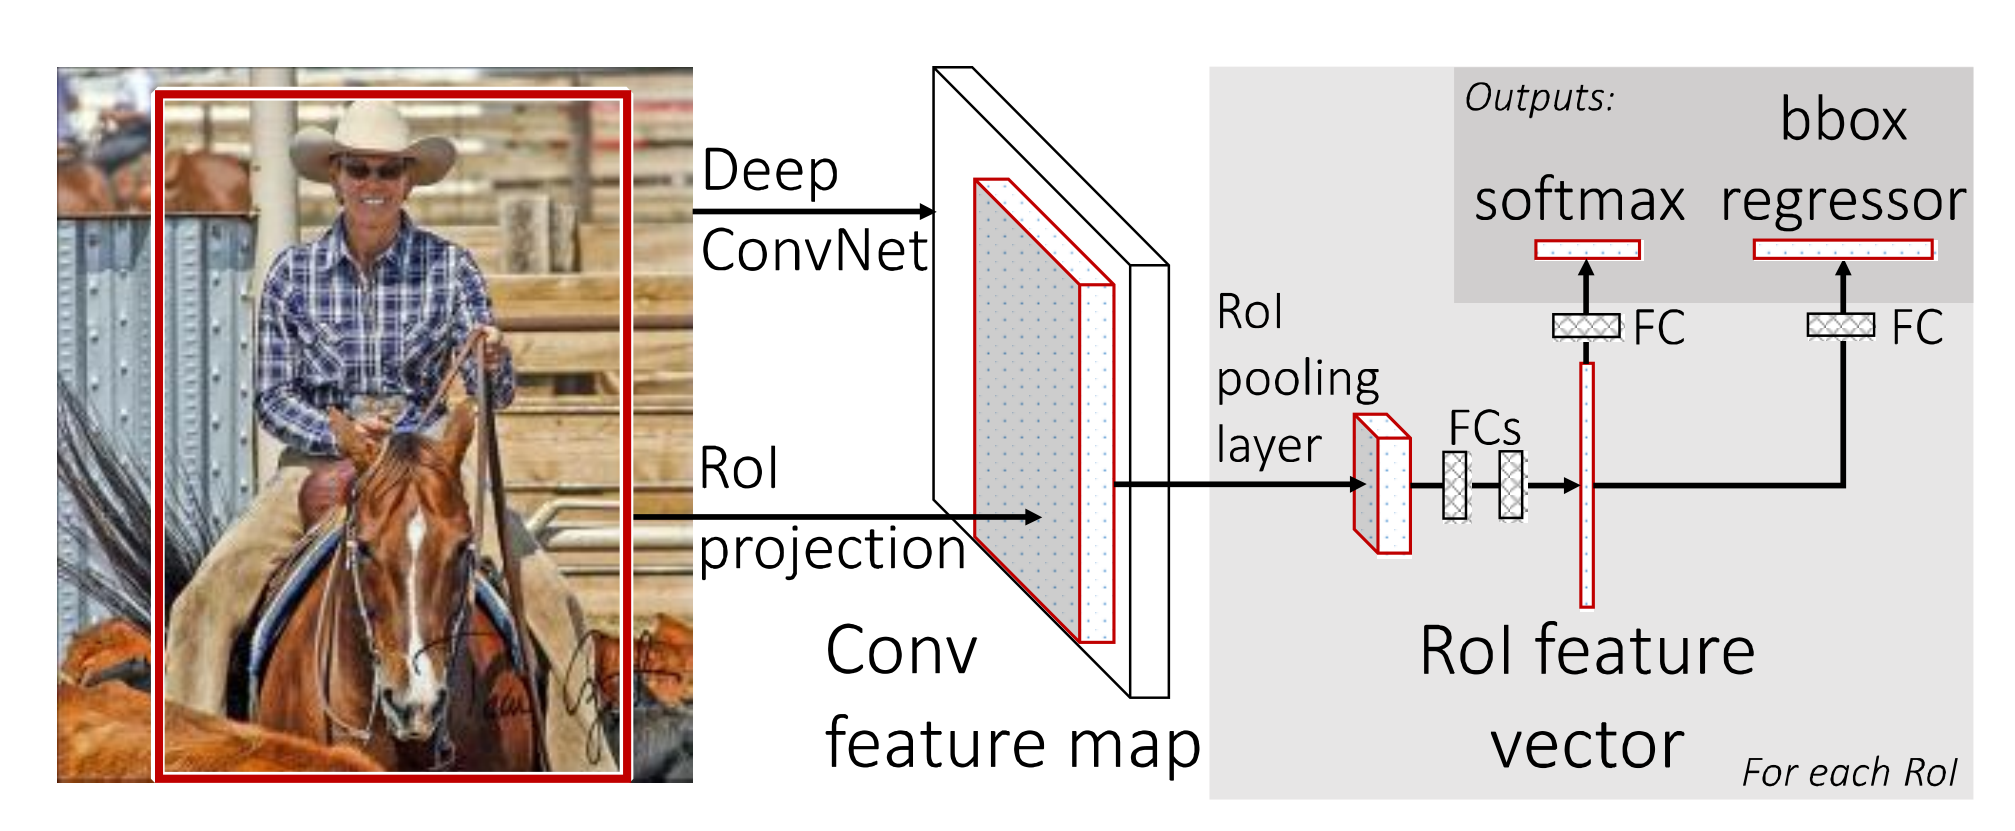
\includegraphics[width=0.7\linewidth]{img/fast_r-cnn_structure}
	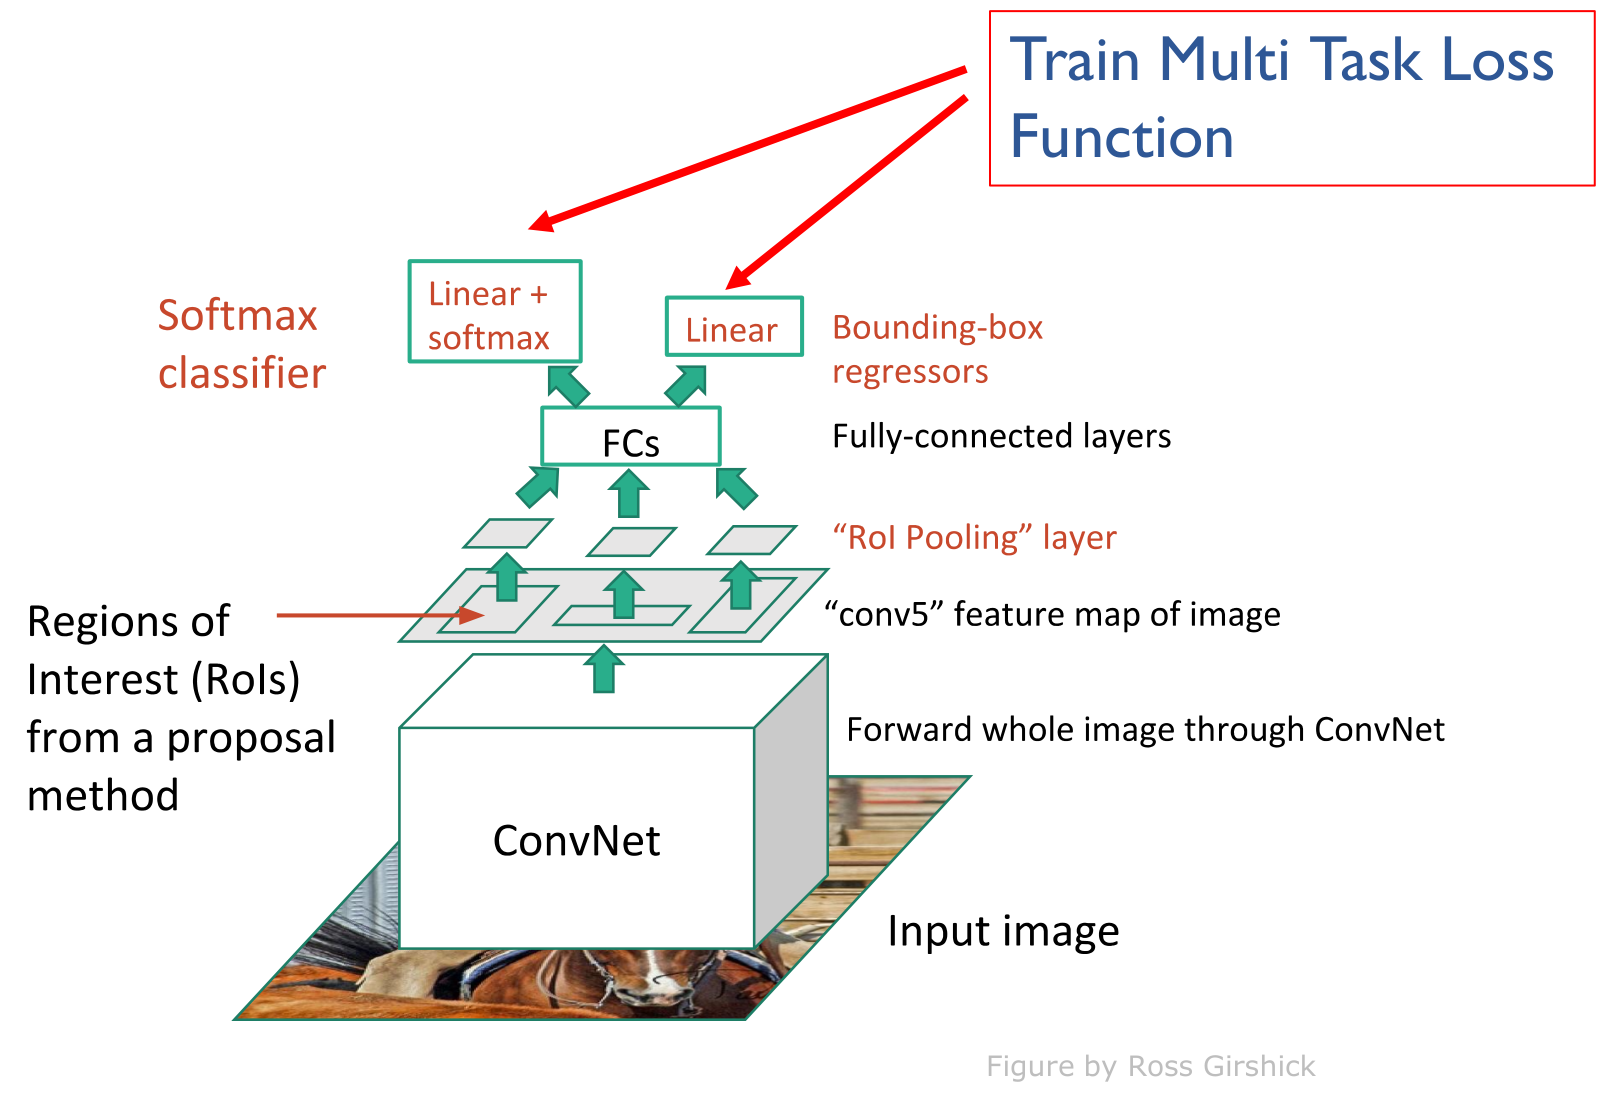
\includegraphics[width=0.7\linewidth]{img/fast_r-cnn_structure2}
\end{figure}

\subsection{You Only Look Once (YOLO)}
YOLO is a single neural network predicting bounding boxes and classification probabilities.
It is fast with good classification but less accurate localization.

\subsubsection{Improvements}
\begin{itemize}
	\item Add Batch Normalization
	\item Use higher resolution ($448\times 448$)
	\item Use Anchor Bounding Boxes from k-Means Analysis on the training data
	\item Use a new base net (darknet19 and darknet 58)
\end{itemize}
